\chapter{Further Properties of the Correspondence}
\label{chap:further_properties}

\chapterquote{Everything is  funny,  if you can laugh at it.}{Lewis Carroll}

The previous chapter introduced the graph-simplex correspondence and devoted several sections to the basic properties of the simplices associated to a given graph. In this chapter we  continue the study of the correspondence and present several of its more significant and advanced properties.  



\section{Block Matrix Equations}
\label{sec:block_matrix}
In this section we present matrix equations pertaining to both hyperacute simplices and the effective resistance of graphs. The equations appeal to the relationship between hyperacute simplices and graphs by using well known results from the literature on electrical networks and effective resistance. The goal of this section is to demonstrate to the reader the utility of the graph-simplex correspondence in generating statements about hyperacute simplices by hijacking our knowledge of graph theory,  and vice versa. 

We begin with a block matrix equation describing some aspects of  the geometry between a  hyperacute simplex and its dual. It is closely related to an equation given by Fiedler in Theorem 1.4.1 in \cite{fiedler2011matrices}. Instead  of a direct proof, we use the results of Van Mieghem \etal~\cite{van2017pseudoinverse} and prove it by leveraging aspects of the effective resistance of a graph.  

Let a centred, hyperacute simplex $\ssplx$ be given, with $\Sv(\ssplx)=\{\bgamma_i\}$.  Let $\bar{d}$ be the average squared distance between all the vertices of $\ssplx$, that is
\begin{equation}
\label{eq:avg_squared_distance}
\bar{d} \equiv  \frac{1}{n^2}\sum_{i\leq j} \norm{\bgamma_i-\bgamma_j}_2^2.
\end{equation}
Let $\xi(i)$ give the average squared distance of vertex $i$ from other vertices minus the total average distance, 
\begin{equation}
\label{eq:avg_sqd_distance_i}
\xi(i) \equiv \frac{1}{n}\sum_{j} \norm{\bgamma_i-\bgamma_j}_2^2 - \bar{d},
\end{equation}
and put $\bxi=(\xi(1),\dots,\xi(n))$. 
Then we have the following result. 

\begin{lemma}
	\label{lem:block_inverse_simplex}
	Let $\ssplx\subset\R^{n-1}$ be a hyperacute simplex with  squared distance matrix $\D$, and average squared distance vector $\bxi$. Denote by $\BGamma$ the vertex matrix of $\ssplx^\du$, the dual simplex to $\ssplx$. Then, 
	\begin{equation}
	\label{eq:simplex_block_matrix}
	-\frac{1}{2} \begin{pmatrix}
	0 & \one_n^\tp \\ 
	\one_n &  \D
	\end{pmatrix} = \begin{pmatrix}
	\bxi^\tp \BGamma^\tp \BGamma\bxi + 4\overline{d} & -(\BGamma^\tp \BGamma\bxi + 2\one/n)^\tp \\
	-(\BGamma^\tp \BGamma\bxi + 2\one/n) & \BGamma^\tp \BGamma
	\end{pmatrix}^{-1}.
	\end{equation}
	Moreover, the vertices $\ssplx^\du$ and the distance matrix of $\ssplx$ are related by the equation
	\begin{equation}
	\label{eq:lem_inverse_relation}
	\BGamma^\tp \BGamma \D \BGamma^\tp \BGamma = -2\BGamma^\tp \BGamma,
	\end{equation}
	and in the space $\spn(\one)^\perp$ it holds that 
	\begin{equation*}
	\label{eq:lem_inverse_relation2}
	\D\BGamma^\tp \BGamma \D= -2\D.	
	\end{equation*}
\end{lemma}

\begin{proof}
As above, $\ssplx$ is the inverse simplex of some graph $G$, and therefore, $\D=\Reff$, where $\Reff$ is the effective resistance matrix. Therefore, we can rewrite $\xi(i)$ as 
\begin{align*}
\frac{1}{n}\sum_j \effr(i,j) - \frac{1}{n^2}\sum_{i<j}\effr(i,j),
\end{align*}
and $\bxi$ as 
\begin{align*}
\bxi = \frac{1}{n}\Reff\one - \frac{1}{n^2} \one \one^\tp \Reff\one = \frac{1}{n}\Reff\one - \frac{1}{n^2} \J \Reff\one.
\end{align*}
Meanwhile, the dual simplex to $\ssplx$ is the simplex of the graph $G$, and hence obeys $\BGamma^\tp\BGamma=\L_G$. Consequently, letting $\u=\frac{1}{n}\Reff\one - \frac{1}{n^2} \J \Reff\one$, we can rewrite Equation \ref{eq:simplex_block_matrix} as the purely graph theoretic statement  
\begin{equation}
\label{eq:block_inverse_er}
	-\frac{1}{2} \begin{pmatrix}
0 & \one_n^\tp \\ 
\one_n &  \Reff
\end{pmatrix} = 
\begin{pmatrix}
\u^\tp \L_G\u + \frac{4}{n^2}R & -(\L_G\u + \frac{2}{n}\one)^\tp \\
-(\L_G\u + \frac{2}{n}\one) & \L_G
\end{pmatrix}^{-1}.
\end{equation}
where $R=\sum_{i<j}\effr(i,j)$ is the total effective resistance in the graph. The above equality was proved by Van Mieghem \etal~\cite{van2017pseudoinverse}, and in a more general form by Fiedler~\cite{fiedler1993geometric,fiedler2011matrices}, but we prove it here for completeness. Multiplying out the left hand side, the top left-hand corner of the resulting block matrix is
\[-\frac{1}{2}(\one^\tp\L_G - \frac{2}{n}\one^\tp \one) = 1,\]
since $\one^\tp \L_G=\one^\tp\L_G^\tp =\zero$. Likewise the top-right hand corner is $\zero$. The bottom left-hand corner is 
\begin{equation}
\label{eq:lem_block_matrix}
-\frac{1}{2}\bigg(\one\bxi^\tp \L_G\bxi +\frac{4}{n^2} R \one - \Reff\L_G\bxi - \frac{2}{n}\Reff\one\bigg),
\end{equation}
where, using that $\Reff=\bxi \one^\tp + \one \bxi^\tp -2\L_G^+$ and $\one^\tp\L_G=\zero$, 
\begin{align}
\Reff\L_G = \one\bxi^\tp \L_G - 2\bigg(\I-\frac{1}{n}\J\bigg).\label{eq:lem_block_matrix2}
\end{align}
Equation \eqref{eq:lem_block_matrix} thus becomes 
\begin{align*}
\frac{1}{n}\Reff\one -\frac{2}{n^2}R \one - \bigg(\I-\frac{1}{n}\J\bigg)\bxi &= \frac{1}{n}\Reff\one - \frac{2}{n^2}R\one - \bigg(\I-\frac{1}{n}\J\bigg)\bigg(\frac{1}{n}\Reff\one - \frac{1}{n^2}\J\Reff\one\bigg) \\
&= -\frac{2}{n^2} R\one + \frac{1}{n^2}\Reff\one + \frac{1}{n^2}\J\Reff\one - \frac{1}{n^3}\J^2\Reff\one \\
&= -\frac{2}{n^2} R\one +\frac{1}{n^2} \J\Reff\one = \zero,
\end{align*}
using that $\J^2 = n \J$, $R=\frac{1}{2}\one^\tp \Reff\one$, and $\J\Reff\one = \one(\one^\tp \Reff\one) = \one R$. Finally, again using \eqref{eq:lem_block_matrix2}, the bottom right-hand side is 
\begin{align*}
\frac{1}{2}\one \bxi^\tp \L_G + \frac{1}{n}\one\one^\tp - \frac{1}{2}\Reff\L_G &= \frac{1}{n}\J + \bigg(\I-\frac{1}{n}\J\bigg) = \I.
\end{align*}
This demonstrates that \eqref{eq:lem_block_matrix} holds. We now show that $\L_G \Reff\L_G = -2 \L_G$ and that $\Reff\L_G\Reff\x = -2\Reff\x$ for all $\x\in\spn(\one)^\perp$, which will complete the proof. Applying Equation \eqref{eq:lem_block_matrix2} we have 
\begin{align*}
\L_G\Reff\L_G = \L_G\one \bxi^\tp\L_G = -2\L_G+ \frac{2}{n}\L_G\one\one^\tp = -2\L_G.
\end{align*}
In the same way as \eqref{eq:lem_block_matrix2} was derived, we see that 
\begin{equation*}
\L_G\Reff = \L_G\bxi\one^\tp - 2\bigg(\I-\frac{1}{n}\J\bigg),
\end{equation*}
and so 
\begin{equation*}
\Reff\L_G\Reff= \bigg(\Reff\L_G\bxi^\tp + \frac{2}{n}\one \bigg)\one^\tp -2\Reff,
\end{equation*}
as desired. 
\end{proof}

Owing to the various connections between graphs and simplices, the block matrix equation has several different flavours. Lemma~\ref{lem:block_inverse_simplex}, for example, provides an interpretation purely in terms of simplices, while Equation~\eqref{eq:block_inverse_er} provides a relationship between the Laplacian, its pseudoinverse, and  the effective resistance of the graph. 
We can combine  these two interpretations to obtain the following relationship between a graph's Laplacian and its inverse (combinatorial) simplex. 

\begin{corollary}
	For a  graph $G$ with inverse simplex $\splx^+$ which has distance matrix  $\D(\splx^+)$, 
	\begin{equation}
	\label{eq:block_inverse_graph_simplex}
	-\frac{1}{2}\begin{pmatrix}
	0 & \one^\tp \\
	\one & \D(\splx_G^+)
	\end{pmatrix} = 
	\begin{pmatrix}
	\u^\tp  \L_G \u  + 4R_G/n^2
	&  -(\L_G\u + \frac{2}{n}\one )^\tp \\
	-(\L_G\u + \frac{2}{n}\one ) 
	& \L_G
	\end{pmatrix}^{-1},
	\end{equation}
	where $\u=\diag(\L_G^+(i,i))$. \note{Add the other relationships.}
\end{corollary}

One consequence of the above is a relation between the volume of the simplex and the effective resistances in the graph. To see this, we need to introduce a particular object from the field of distance geometry. Let $\D(\X)$ be the distance matrix of a set $\X$ of $d$ points. The matrix 
\begin{equation}
\label{eq:menger_matrix}
\begin{pmatrix}
0 & \one^\tp \\
\one & \D(\X)
\end{pmatrix}\in\R^{(d+1)\times (d+1)},
\end{equation}
is called the \emph{Menger matrix of $X$}, the determinant of which is called the \emph{Cayley-Menger determinant}, named after Arthur Cayley and Karl Menger~\cite{cayley1841theorem, Menger1928}. The Cayley-Menger determinant is related to the volume of the underlying set of points as follows. 


\begin{lemma}[\cite{menger1931new}]
	\label{lem:menger_volume}
	Let $\D(\X)$ be the distance matrix of a set $\X$ of $d$ points. The squared $d-1$ dimensional volume\footnote{That is, the volume as calculated in $\R^{d-1}$.} of the convex hull of $\X$ is proportional to the root of the determinant of the Menger matrix: 
	\begin{equation}
	\label{eq:vol(convX)}
	\vol^2(\conv(\X)) = \frac{(-1)^d}{((d-1)!)^2 2^{d-1}} \det\begin{pmatrix}
	0 & \one^\tp \\
	\one & \D(\X)
	\end{pmatrix}.
	\end{equation} 
\end{lemma}

The relation between the Menger matrix and the volume combined with the matrix equations above, allows us to give a concise formula for the volume of any hyperacute simplex. This was first pointed out in \cite{van2017pseudoinverse}. 

\begin{lemma}
	\label{lem:volume}
	Let $\ssplx\subset\R^{n-1}$ be a hyperacute simplex, and let $G$ be its associated graph. Then $\ssplx$'s $n-1$ dimensional volume is 
	\begin{equation}
	\label{eq:vol(T)}
	\vol(\ssplx) = \frac{1}{(n-1)!\cdot \Gamma_G^{1/2}},
	\end{equation}
	where $\Gamma_G$ is the total weight of all spanning  trees of $G$. 
\end{lemma}

We remind the reader that $\Gamma_G$ was discussed in  Section~\ref{sec:background_laplacian}; see  Equation~\ref{eq:Gamma_G}  in particular. The proof of Lemma~\ref{lem:volume} may  be  found in Appendix~\ref{sec:app_proofs_further}.   


We can use these results to produce a surprising equation concerning  the diagonal entries of the Laplacian. In particular, $\L_G(i,i)$ is proportional to the ratio of the weight of  spanning trees in $G$ to this weight when the vertex $i$ is removed. 

\begin{lemma}
	\label{lem:L(i,i)_trees}
	Let $G$ be a connected graph and fix $i\in V(G)$. 
	The Put $G_\ic=G[V\setminus \{i\}]$. The diagonal entries of the combinatorial Laplacian are given by 
	\begin{equation}
	\label{eq:L(i,i)_trees}
	\L_G(i,i) = \frac{\Gamma_G}{\Gamma_{G_\ic}}.
	\end{equation}
	Moreover, if $\splx^+\subset\R^{n-1}$  is the inverse combinatorial simplex of $G$ then the volumes
	of $\splx^+_\ic$ and $\splx^+$ are related as 
	\begin{equation}
	\label{eq:vol/vol}
	\frac{\vol^2(\splx_\ic^+)}{\vol^2(\splx^+)} = (n-1)^2\L_G(i,i). 
	\end{equation}
\end{lemma}
\begin{proof}
	We will begin with Equation~\eqref{eq:vol/vol}. 
	Let $\splx^+$ have vertices $\sv_1^+,\dots,\sv_n^+$, and let $\M$ be the Menger matrix associated with $\splx^+$. Sylvester's formula (Lemma~\ref{lem:sylvester}) gives us that 
	\begin{equation*}
	\M^{-1}(i+1,i+1) =\det\M^{-1}(i+1,i+1)= \pm \frac{\det\M(U,U)}{\det\M},
	\end{equation*}
	where $U=\{i+1\}^c$. Observe that $\M(U,U)$ is the Menger matrix of the simplex $\splx_\ic$; we are simply removing the row and column corresponding to the $i$-th vertex. Translating the determinants of Menger matrices into statements about volumes of simplices via Equation~\eqref{eq:vol(T)} gives 
	\begin{align*}
	\M^{-1}(i+1,i+1) &= \pm \frac{[(n-2)!]^2 2^{n-2}}{(-1)^{n-1}}\vol^2(\splx_\ic^+) \bigg / \frac{[(n-1)!]^2 2^{n-1}}{(-1)^n} \vol^2(\splx^+) \\
	&= \mp \frac{1}{2(n-1)^2}\frac{\vol^2(\splx_\ic^+)}{\vol^2(\splx^+)}. 
	\end{align*} 
	Via the block matrix equation \eqref{eq:block_inverse_graph_simplex} we have $\M^{-1}(i+1,i+1) = -\frac{1}{2}\L_G(i,i)$. Plugging this into the above equation and noting that both $\L_G(i,i)$ and $\vol^2(\splx_\ic^+)/(2n^2\vol^2(\splx^+))$ are positive  gives the desired result. 
	Equation~\eqref{eq:L(i,i)_trees} now comes from writing out the  simplex volumes $\vol(\splx_\ic^+)$ and $\vol(\splx^+)$ in terms of spanning trees of $G$ by \eqref{eq:vol(T)}, after using \eqref{eq:vol/vol}:
	\begin{align*}
	\L_G(i,i)  &= \frac{\vol^2(\splx^+_\ic)}{(n-1)^2\vol^2(\splx^+)} = \frac{1}{(n-2)!^2\cdot \Gamma_{G[\ic]}} \bigg/ \frac{(n-1)^2}{(n-1)!^2\cdot \Gamma_G} = \frac{\Gamma_{G}}{\Gamma_{G[\ic]}}.\qedhere
	\end{align*}
\end{proof}

\begin{corollary}
	For all $i\in[n]$, the length of the vertex vector $\sv_i$ of $\splx_G$ obeys
	\begin{equation}
	\label{eq:||sv_i||_vol}
	\norm{\sv_i}_2^2 = \frac{\Gamma_G}{\Gamma_{G[\ic]}} = \frac{\vol^2(\splx_\ic^+)}{(n-1)^2\vol^2(\splx^+)}.
	\end{equation}
\end{corollary}
\begin{proof}
	Follows immediately from Lemma~\ref{lem:L(i,i)_trees}. 
\end{proof}

\begin{lemma}
	\label{lem:volT_multi}
	For any hyperacute simplex $\ssplx\subset\R^{n-1}$ and  $i\in[n]$, the following equations hold:
	\begin{enumerate}
		\item $\vol(\ssplx_\ic) = \sum_{j\neq i}\vol(\ssplx_\jc)\cos\theta_{ij}(\ssplx)$;
		\item $\vol^2(\ssplx_\ic) =  \sum_{j\neq i}\vol^2(\ssplx_\jc) - \sum_{j,k\neq i,j\neq k} \vol(\ssplx_\jc)\vol(\ssplx_\kc)\cos\theta_{jk}(\ssplx)$; and
		\item $(n-1)\vol(\ssplx_{\{i,j\}^c})\vol(\ssplx) = (n-2)\vol(\ssplx_\ic)\vol(\ssplx_\jc)\sin\theta_{ij}(\ssplx)$ for  all $j\neq i$. 
	\end{enumerate}
	Here, as usual, $\theta_{ij}(\ssplx)$ is the angle between $\ssplx_\ic$ and $\ssplx_\jc$. 
\end{lemma}

\begin{remark}
	One might expect that the second equation in the above lemma follows immediately from squaring the first. However, performing the computation demonstrates that this is not the case. Hence the second equation is in  fact providing new information. 
\end{remark}
\begin{proof}
	It suffices to take $\ssplx=\splx^+$, the  inverse combinatorial simplex of some graph $G$.  Let $\{\sv_i\}$ be the vertices of $\splx_G$, the combinatorial simplex of $G$. 	
	We have $\L_G(i,j)=\la\sv_i,\sv_j\ra = \norm{\sv_i}_2\norm{\sv_j}_2\cos\phi_{ij}$, where $\phi_{ij}$ is the angle between $\sv_i$ and $\sv_j$. Since the vertices $\{\sv_i\}$ are  dual to those of $\splx^+_G$, we have $\cos\phi_{ij}=-\cos\theta^+_{ij}$ where $\theta^+_{ij}$ is the angle between $\splx^+_\ic$ and $\splx^+_\jc$. (We are applying the same reasoning here as in Sections~\ref{sec:background_simplex_angles} and~\ref{sec:simplex_to_graph}.) Combining this with the fact that $\L_G\one=\zero$ and Equation~\eqref{eq:||sv_i||_vol} gives
	\begin{align*}
	0 &= \sum_{j\in[n]} \L_G(i,j) = \norm{\sv_i}_2^2 - \sum_{j\neq i}\norm{\sv_i}_2\norm{\sv_j}_2\cos\theta_{ij}^+ \\
	&= \frac{\vol(\splx_\ic^+)}{n^2\vol^2(\splx^+)} \bigg(\vol(\splx^+_\ic) - \sum_{j\neq i}\vol(\splx_\jc^+)\cos\theta_{ij}^+\bigg),
	\end{align*}
	which proves the first equation. To see the second,  note that $\L_G(i,k)=-\sum_{j\neq k}\L_G(i,k)$  (again using that $\L_G\one=\zero$). Applying  this twice, we obtain 
	\[\L_G(i,i) = -\sum_{j\neq i}\L_G(i,j) = \sum_{j\neq i}\sum_{k\neq i}\L_G(k,j) = \sum_{j\neq i}\L_G(j,j) + \sum_{j,k\neq i,k\neq j}\L_G(k,j).\] 
	As above,  translating this to expressions involving the volumes of facets of $\splx^+$ and then multiplying through by $n^2\vol(\splx^+)$ gives  
	\begin{equation*}
	\vol^2(\splx_\jc^+) = \sum_{j\neq i}\vol^2(\splx_\jc^+) - \sum_{j,k\neq i,k\neq j} \vol(\splx_\kc^+)\vol(\splx_\jc^+)\cos\theta_{kj}^+. 
	\end{equation*}
	It remains to  prove  the  third equation.  Let $\M$ be  the Menger matrix of $\splx^+$, and  let $U=\{i,j\}$  and  $U_1=\{i+1,j+1\}$ for any $i\neq j$. Without loss of generality assume  $i<j$. 
	Notice that $\M(U_1^c,U_1^c)$ is the Menger matrix of the vertices $\{\sv_k\}_{k\neq i,j}$. 
	Combining Sylvester's equation and our usual block matrix relation gives 
	\begin{align*}
	\frac{\det\M(U_1^c,U_1^c)}{\det \M} &= \pm \det \bigg(-\frac{1}{2}\L_G(U,U)\bigg) \\
	&= 
	\pm \frac{1}{4}\det\begin{pmatrix}
	\norm{\sv_i}_2^2 & \la \sv_i,\sv_j\ra \\
	\la \sv_i,\sv_j\ra & \norm{\sv_j}_2^2 
	\end{pmatrix} \\
	&=\pm \frac{1}{4}\norm{\sv_i}_2^2\norm{\sv_j}_2^2 - \la \sv_i,\sv_j\ra^2 \\
	&= \pm\frac{1}{4}\norm{\sv_i}_2^2\norm{\sv_j}_2^2(1 - \cos^2\phi_{ij})
	\end{align*}
	where $\phi_{ij}$ is the angle between $\sv_i$ and $\sv_j$ (Section~\ref{sec:background_simplex_angles}). Since the vertices $\{\sv_i\}$ are the  duals  to those in $\splx^+$, we have $\cos\phi_{ij}=-\cos\theta_{ij}^+$  so \[\norm{\sv_i}_2^2\norm{\sv_j}_2^2(1 - \cos^2\phi_{ij}) = \norm{\sv_i}_2^2\norm{\sv_j}_2^2(1 - \cos^2\theta_{ij}^+) =  \norm{\sv_i}_2^2\norm{\sv_j}_2^2\sin^2\theta_{ij}^+.\]   
	Writing $\det\M(U_1^c,U_1^c)$  in terms of $\vol\splx_{U^c}^+$ and $\det \M$  in terms of $\vol\splx^+$ by  means of Equation~\eqref{eq:vol(convX)}, and using Equation~\eqref{eq:||sv_i||_vol} to relate $\norm{\sv_i}_2^2$ and $\norm{\sv_j}_2^2$  to  the volumes of $\splx_\ic^+$  and $\splx_\jc^+$ then yields 
	\begin{align*}
	\frac{1}{4(n-1)^2(n-2)^2}\frac{\vol^2\splx_{U^c}^+}{\vol^2\splx^+} =  \frac{\vol^2\splx_\ic^+}{(n-1)^2\vol^2\splx^+}\frac{\vol^2\splx_\jc^+}{(n-1)^2\vol^2\splx^+}\sin^2\theta_{ij}^+.
	\end{align*}
	Notice that we have rid ourselves  of the ambiguity in sign because we see that both  sides are the square of some quantity, hence are  positive. 
	Simplying and taking the square root of both sides of the above expression gives the third equation.
\end{proof}





Our next set of results demonstrate the the inverse relation can be used not only to infer geometric properties of simplices, but also graph-theoretic properties. A variant of the following  was proved by Fiedler~\cite{fiedler2011matrices}. 

\begin{lemma}
	\label{lem:block_matrix_tree}
 For a weighted and connected tree $T=(V,E,w)$ on $n$ vertices let the matrix $\bS_T$ describe the inverse distances  between vertices, i.e., for $(i,j)\in E$, $\bS_T(i,j) = 1/w(i,j)$ and for $(i,j)\notin E$, $\bS_T(i,j) = \sum_{\ell=1}^{k-1} 1/w(v_\ell,v_{\ell+1})$ where $i=v_1,v_2,\dots,v_k=j$ is the unique path between $i$ and $j$. Then,
 \begin{equation}
 \label{eq:block_ST}
-\frac{1}{2} \begin{pmatrix}
0 & \one^\tp \\
\one & \bS_T 
\end{pmatrix}
\begin{pmatrix}
\sum_{i\sim j}1/w(i,j)  & (\d-2\one)^\tp \\
\d-2\one & \L_T
\end{pmatrix} = \I.
 \end{equation}
\end{lemma}

\begin{corollary}
	Let $T$  be a weighted and connected tree. Then 
	\begin{equation*}
	\bxi^\tp \L_T\bxi + \frac{4R_T}{n^2} = \sum_{i,j}  \frac{1}{w(i,j)}, \quad \text{and}\quad \L_G\bxi = \bigg(2-\frac{2}{n}\bigg)\one - \d,
	\end{equation*}
	where $\bxi = \diag(\L_T^+(i,i))=\frac{1}{n}\Reff\one - \frac{1}{n^2} \J \Reff\one$ and $\d= (\deg(1),\dots,\deg(n))$. 
\end{corollary}
\begin{proof}
	Let $\bS_T$ be as it was in  Lemma \ref{lem:block_matrix_tree}. It's well known  that in trees, the effective resistance between nodes $i,j$  is equal to $\sum_{s=1}^{r-1} 1/w(v_s,v_{s+1})$ where $i=v_1,\dots,v_r=j$ is the shortest path between $i$ and $j$ in $T$ (see e.g., \cite{ellens2011effective}). That is, $\Reff_T=\bS_T$. Since matrix inverses are unique, combining Equations \eqref{eq:block_ST} and \eqref{eq:block_inverse_graph_simplex} yields 
	\begin{equation*}
	\begin{pmatrix}
	\sum_{i\sim j}1/w(i,j)  & (\d-2\one)^\tp \\
	\d-2\one & \L_T
	\end{pmatrix} = \begin{pmatrix}
\bxi^\tp  \L_T \bxi  + 4R_T/n^2
	&  -(\L_T\bxi + \frac{2}{n}\one )^\tp \\
	-(\L_T\bxi + \frac{2}{n}\one ) 
	& \L_T
	\end{pmatrix},
	\end{equation*}  
	from which the claim follows. 
\end{proof}






\section{Inequalities}
\label{sec:inequalities}
In this section we demonstrate how the graph-simplex may be used to obtain both geometric and graph-theoretic inequalities. We begin with an inequality relating the quadratic form $\Lf$ to the ``weight'' of the cuts associated with the pseudoinverse.  It was first proved by Devriendt and Van Mieghem~\cite{devriendt2018simplex}. Interestingly, a parallel result for the normalized Laplacian form does not seem to exist. 
 
\begin{lemma}
	\label{lem:ineq_f1}
For any $f$ with $\la f,\one\ra=0$, $
\Lf(f) \geq \norm{f}_1^2/4w(\partial^+F^+)$, 
for $F^+\equiv \{i:f(i)\geq 0\}$. 
\end{lemma}

Given the combinatorial simplex $\splx_G$ of the  graph $G$, it has a natural corresponding normalized simplex, namely $\splxn_G$. Using Cheeger's inequality~\cite{chung1997spectral}
\begin{equation*}
\cond_G \geq \lambdan_{n-1} \geq \frac{\cond_G^2}{2},
\end{equation*}  
where  $\lambdan_1\geq \lambdan_{n-1}>\lambdan_n=0$ are the eigenvalues of the normalized Laplacian of  $G$, and $\cond_G$ is the \emph{conductance of $G$}, 
\begin{equation*}
\cond_G\equiv \min_{U:vol(U)\leq \vol(G)/2} \frac{\vol(\partial U)}{|U|},
\end{equation*}
we can  relate  the centroids of $\splx_G$ to $\splxn_G$ as follows. 

\begin{observation}
	\begin{equation*}
	\min_{U:\vol(U)\leq \vol(G)/2} \norm{\cent(\splx_U)}_2^4 |U|^2  \leq \min_{i=1}^n (\Svn\Svn^\tp)(i,i) \leq \min_{U:\vol(U)\leq \vol(G)/2} \norm{\cent(\splx_U)}_2^2 |U|.  
	\end{equation*}
\end{observation}
\begin{proof}
	Use that $\norm{\cent(\splx_U)}_2^2 =  |U|^{-2} \bchi_U\L_G\bchi_U$ (Section~\ref{sec:S_G}) and that $\Svn\Svn^\tp=\Evaln$ (Equation~\eqref{eq:SvSv^t}) and apply Cheeger's inequality. 
\end{proof}

We can translate several of the results obtained in the previous section on  volumes and spanning  into inequalities. 

\begin{lemma}
\label{lem:volT_inequalities}
For any hyperacute simplex $\ssplx\subset\R^{n-1}$ and  $i\in[n]$, the following equations hold:
\begin{enumerate}
	\item $\vol\ssplx_\ic \leq \sum_{j\neq i}\vol\ssplx_\jc$;
	\item $\sum_{j\neq i}\vol^2\ssplx_\jc\geq \vol^2\ssplx_\ic\geq   \sum_{j\neq i}\vol^2\ssplx_\jc - \sum_{j,k\neq i,j\neq k} \vol\ssplx_\jc\vol\ssplx_\kc$; and
	\item $(n-1)\vol\ssplx_{\{i,j\}^c}\vol\ssplx \leq  (n-2)\vol(\ssplx_\ic)\vol(\ssplx_\jc)$ for  all $j\neq i$.
\end{enumerate}
\end{lemma}
\begin{proof}
	Follows immediately from Lemma~\ref{lem:volT_multi} after  recalling that because $\ssplx$  is  hyperacute all interior  angles are at most $\pi/2$. We remark that for the second  equation  we have simply provided the  easy  upper bound provided by Equation 2 of Lemma~\ref{lem:volT_inequalities}. 
\end{proof}

More interestingly  however,  we can use the relation between volume of a  graph's inverse combinatorial s simplex and the weight of its spanning trees (Equation~\eqref{eq:vol(T)})  to give inequalities pertaining to the latter.  

\begin{lemma}
	\label{lem:tree_inequalities}
	For any weighted,  connected  graph  $G$ and all $i\in V(G)$, 
	\begin{enumerate}
		\item $\Gamma_{G_\ic}^{-1/2} \leq \sum_{j\neq i}\Gamma_{G_\jc}^{-1/2}$;
		\item $\sum_{j\neq i}\Gamma_{G_\jc}^{-1} \geq \Gamma_{G_\ic}^{-1} \geq \sum_{j\neq i}\Gamma_{G_\jc}^{-1} - \sum_{j,k\neq i,j\neq k}\Gamma_{G_\jc}^{-1/2}\Gamma_{G_\kc}^{-1/2}$; and 
		\item $\Gamma_{G_\ic}\Gamma_{G_\jc}\leq \Gamma_{G_{\{i,j\}^c}}\Gamma_G$ for all $j\neq i$. 
	\end{enumerate}
\end{lemma}
\begin{proof}
	All  equations follow from applying Lemma~\ref{lem:volT_inequalities}  together with Equation~\ref{eq:vol(T)} and simplifying. 
\end{proof}

\note{Still working on this content. Since $\Reff_G=n\sum_i\lambda_i^{-1}=n\tr(\Sv\Sv^\tp)$,
facts/inequalities pertaining to the effective resistance can be translated to the simplex. }



\section{Quadrics}
\label{sec:quadrics}

Here we explore several quadrics associated with the simplices of $G$. 
We remind the reader that a  \emph{quadric} in $\R^d$ is a hypersurface of dimension $d-1$ of the form 
\begin{equation*}
\{\x\in\R^d: \x^\tp \Q\x + \r^\tp \x + s=0\},
\end{equation*}
for some $\Q\in\R^{d\times d},\r\in\R^d$  and $s\in \R$. 
In $\R^3$, typical examples of quadrics are spheroids and ellipsoids ($\r=\zero$ in these cases), paraboloids, hyperboloids, and  cylinders. In what follows we focus on ellipsoids, in particular on \emph{circumscribed} ellipsoids. Such a quadric of interest in simplex geometry is the following. 

\begin{definition}[\cite{krause1983steinerellipsoide}]
\label{def:steiner_ellipsoid}
The \emph{Steiner Circumscribed Ellipsoid}, or simply the \emph{Steiner Ellipsoid} of a simplex $\splx$ with vertices $\{\sv_i\}$ is a quadric which contains the vertices and whose tangent plane at $\sv_i$ is parallel to the affine plane spanned by $\{\sv_j\}_{j\neq i}$. 
\end{definition}

Its existence  and uniqueness is guaranteed by the following theorem. 

\begin{theorem}[\cite{fiedler2005geometry}]
The Steiner ellipsoid of a simplex $\splx$ is unique and moreover, is the ellipsoid with minimum volume which contains $\splx$. 
\end{theorem}

Owing to its uniqueness, we denote the Steiner ellipsoid of the simplex $\splx$ by $\El(\splx)$. The following lemma gives an explicit representation of the circumscribed ellipsoid of the combinatorial simplex of $G$---which we will  henceforth call the \emph{(Steiner) circumscribed ellipsoid of $G$}---and of its inverse, which we call the \emph{inverse (Steiner) circumscribed Ellipsoid of $G$}. 

\begin{lemma}[\cite{fiedler2005geometry}]
	\label{lem:El(S)}
The Steiner circumscribed ellipsoid  of $G$ and its inverse  are described by 
\begin{equation}
\label{eq:steinerE}
    \El(\splx_G) = \bigg\{\x: \x^\tp \Sv^+(\Sv^+)^\tp \x - \frac{n-1}{n}=0\bigg\},
\end{equation}
and 
\begin{equation}
\label{eq:steinerE_inverse}
\El(\splx^+_G) = \bigg\{\x: \x^\tp \Sv\Sv^\tp \x - \frac{n-1}{n}=0\bigg\}.
\end{equation}
\end{lemma}


 Perhaps a more insightful representation of $\El(\splx)$ comes from appealing to Equation \eqref{eq:SvSv+}, i.e., $\Sv\Sv^\tp = \Eval^{-1/2}$. Hence, by \eqref{eq:steinerE},
\begin{equation}
\label{eq:steinerE2}
    \El(\splx) = \bigg\{\x:\x^\tp \Eval^{-1}\x = \frac{n-1}{n}\bigg\}.
\end{equation}

This allows us to give explicit formulas for the semi-axes of $\El(\splx)$.
 The \emph{semi-axes} of an ellipsoid written in the standard form $\x^\tp \D^2\x=1$ with $\D\in\R^{d\times d}$ a diagonal matrix are the $d$ vectors $\e_i\cdot \D(i,i)^{-1}$. They are the unique vectors $\u_i$ such that any  point $\x$ on the ellipsoid can be written as $\x=\sum_i \u_i\alpha_i$ with  $\sum_i\alpha_i^2=1$~\cite{devriendt2018simplex}. 
 
 \begin{lemma}
 	The semi-axes of the Steiner Cirscumscribed Ellipsoid  $\El(\splx_G)$ of  the graph $G$ are 
 	\[\frac{\e_i}{\sqrt{\lambda_i} }\cdot \bigg(\frac{n}{n-1}\bigg)^{1/2}, \]
 	for $i=1,\dots,n-1$. 
 \end{lemma}
\begin{proof}
	The diagonal matrix $\D=\Eval^{-1/2} (\frac{n}{n-1})^{1/2}$ has entries $D(i,i) = \e_i(\frac{n}{(n-1)\lambda_i})^{1/2}$, and equation  \eqref{eq:steinerE2} demonstrates  that  $\El(\splx_G) = \{\x:\x^\tp \D^2\x=1\}$. Apply the definition of semi-axes. 
\end{proof}

Next we investigate the circumscribed sphere of the combinatorial  simplex. Similarly to the circumscribed ellipsoid, the \emph{cirscumscribed sphere  of a convex body $\P$} is the sphere whose boundary contains all the vertices of $\P$. The circumscribed sphere does not exist in general. However, just as it is possible to always draw a circle containing the endpoints  of a triangle, so the circumscribed sphere of a hyperacute simplex always exists  as is demonstrated  by the following lemma.  

\begin{lemma}[\cite{fiedler1993geometric}]
	\label{lem:circ_sphere}
	Let $\splx^+\subset\R^{n-1}$ be a hyperacute simplex. The circumscribed sphere  of $\splx^+$ exists and is given by the set of points $\{\x:\x=\Sv\balpha, \; \la \balpha,\one \ra = 1, \; \la \balpha,\D\balpha\ra =0\}$, which is a sphere centred at the point $\frac{1}{2}\Sv(\L_G\bxi + \one/n)$ with radius $\frac{1}{2}\sqrt{\bxi^\tp\L_G\bxi + 4R_G/n^2}$ where $G$ is $\splx^+$'s associated graph, and $\bxi = \diag(\L_G^+(i,i))$. 
\end{lemma}

Until this point, we have been examining only the quadrics associated with the combinatorial simplices. We now consider the normalized simplices. Since all the vertices of the normalized simplex lie on the unit sphere, it's clear  that the circumscribed sphere of $\splxn_G$ is precisely $\{\x:\x^\tp\x=1\}$. It's not as straightforward  to see what they circumscribed ellipsoid, $\El(\splxn)$, is on the other hand. One might suspect that it obeys the  equation $\x^\tp \Svn+(\Svn^+)^\tp=1-1/n$, as this is the natural analogue of \eqref{eq:steinerE}. However, because $\Svn^+$ and $\Svn$ obey a non-constant pseudoinverse relation, this equation fails the first test: $\svn_i^\tp\Svn^+(\Svn^+)^\tp\svn_i = \bchi_i^\tp(\I-\sqrt{\w}\sqrt{\w}^\tp/\vol(G))\bchi_i=1-\sqrt{w(i)w(j)}/\vol(G)$ is non-constant. 
However, at this point we recall that beyond being simply  the inverse simplex of $\splx$, $\splx^+$ is also its dual.  We might thus hazard a guess that the correct matrix is $\Svn^\du (\Svn^\du)^\tp$, where $\Svn^\du$ is the vertex matrix of $\splxn^\du$. This is in fact correct, but to see this we first need to demonstrate that any set of simplex vertices and their  duals obey the same relationship as do the vertices of the combinatorial simplex and its inverse. 

\begin{lemma}
	\label{lem:dot_dual_vertices}
	Let  $\ssplx\subset\R^{n-1}$ be any simplex, and $\ssplx^\du$ its dual, where $\Sv=\Sv(\ssplx)=(\bgamma_i)$ and $\Sv^\du=\Sv(\ssplx^\du)=(\bgamma^\du_i)$. 
	For all $i,j\in[n]$, $\la \bgamma_i,\bgamma_j^\du\ra=\delta_{i,j}-1/n$. 
\end{lemma}
\begin{proof}
	By definition of the dual simplex, for all $i,j\neq n$, $\la \bgamma_i,\bgamma^\du_j-\bgamma^\du_n\ra = \delta_{ij}$. Recalling that $\bgamma^\du_n=-\sum_{\ell<n}\bgamma^\du_\ell$, write 
	\begin{align*}
	\la \bgamma_i,\bgamma^\du_n\ra &= - \sum_{\ell<n}\la \bgamma_i,\bgamma^\du_\ell\ra \\
	&= -\sum_{\ell<n} \delta_{i,\ell} + \la \bgamma_i,\bgamma^\du_n\ra \\
	&= -1 - (n-1)\la\bgamma_i,\bgamma^\du_n\ra.
	\end{align*}
	Rearranging the above yields $\la \bgamma_i,\bgamma^\du\ra = -1/n$. Therefore, $\la \bgamma_i,\bgamma^\du_j\ra = \delta_{ij} - 1/n$. It remains to show that $\la\bgamma_n,\bgamma^\du_n\ra=1-1/n$. Proceeding as above, we have 
	\begin{align*}
	\la\bgamma_n,\bgamma^\du_n\ra &= -\sum_{\ell<n}\la \bgamma,\bgamma^\du_\ell\ra = -\sum_{\ell<n} \frac{-1}{n} = \frac{n-1}{n}.\qedhere
	\end{align*}
\end{proof}


From this we can extract the equations of $\El(\splxn)$ and $\El(\splxn^+)$. 

\begin{corollary}
	\label{cor:El(Sn)}
	The normalized Steiner ellipsoid of $G$ is 
	\begin{equation*}
	\El(\splxn) = \bigg\{\x:\x^\tp \Svn^\du(\Svn^\du)^\tp\x = \frac{n-1}{n}\bigg\},
	\end{equation*}
	and the inverse is 
	\begin{equation*}
		\El(\splxn) = \bigg\{\x:\x^\tp (\Svn+)^\du((\Svn^+)^\du)^\tp\x = \frac{n-1}{n}\bigg\}.
	\end{equation*}
	where $\Svn^\du$ contains the vertices of $\splxn_G^\du$ and $(\Svn^+)^\du$ those of $(\splxn_G^+)^\du$. 
\end{corollary}
\begin{proof}
	The computation is almost identical to that in the proof of Lemma~\ref{lem:El(S)}.
\end{proof}



\section{Resistive Polytope}
\label{sec:resistive_polytope}
In this section we explore the relationship between the inverse combinatorial simplex of $G$ and another geometric object related to the effective resistance of the graph. Consider the vertices $\bmu_i=\L_G^{+/2}\bchi_i\in\R^n$, for $i\in[n]$. This yields $n$ points in $\R^n$, also with pairwise squared distances equal to the effective resistance of the graph: 

\begin{equation*}
\norm{\bmu_i-\bmu_j}_2^2 = \norm{\L_G^{+/2}(\bchi_i-\bchi_j)}_2^2 =  (\bchi_i-\bchi_j)^\tp \L_G^+(\bchi_i-\bchi_j)=\effr(i,j).
\end{equation*}

This embedding has been referred to as a \emph{resistive embedding}~\cite{shayanNotes,ding2011cover}, and is an example of an $\ell_2^2$ metric~\cite{arora2009expander} owing  to the well known fact that the effective resistance is a metric (e.g., ~\cite{klein1993resistance}). That being said however, while the mapping seems to be known~\cite{ghosh2008minimizing}, there is very little literature on its properties. 

We  set 
\begin{equation}
\label{eq:res_pol}
\respol_G \equiv \conv(\{\mu_i\}),
\end{equation}
and  call  $\respol_G$ the \emph{resistive polytope of $G$}. Note that $\L_G^{+/2}$ is $\respol_G$'s vertex matrix. As usual, we may omit the subscript $G$ for convenience. We emphasize that while the vertices $\{\bmu_i\}$ obey the same pairwise  distances as  those of the inverse simplex $\splx_G^+$, $\respol_G$  is not the same object as $\splx_G^+$. First, of course, there is  the fact that it sits in  $\R^n$. However,  we also note that the entries of $\mu_i$ (the first $n-1$, at least) do not match those of $\sv_i^+$. Indeed, 

\begin{align*}
\mu_i(\ell) = \L_G^{+/2}(\ell,i) = \sum_{j\in[n]}\lambda_j^{-1/2}\vp_j\vp_j^\tp(\ell,i) = \sum_{j\in[n]}\lambda_j^{-1/2}\vp_j(\ell)\vp_j(i).
\end{align*}
Recalling the formula for the vertices of the inverse simplex $\splx^+$ demonstrates that 
\begin{equation*}
\mu_i(\ell) = \sum_{j\in[n]}\sv_\ell^+(j)\vp_j(i) = \sum_{j\in[n]}\sv_i^+(j)\vp_j(\ell).
\end{equation*}
Hence, in general, $\mu_i(\ell)\neq \sv_i^+(\ell)$. However, the dot products between the vertices of $\respol_G$ does respect  the same relationships as those between the vertices of $\splx_G^+$:
\begin{align*}
\la \bmu_i,\bmu_j\ra &=\sum_{\ell\in[n]} \L_G^{+/2}(\ell,i)\L_G^{+/2}(\ell,j) \\
&= \la \L_G^{+/2}(\cdot,i),\L_G^{+/2}(\cdot,j)\ra \\
&=\la \L_G^{+/2}(\cdot,i),\L_G^{+/2}(j,\cdot)\ra= \L_G^+(i,j),
\end{align*}
since $\L_G^{+/2}$ is symmetric and  $\L_G^{+/2}\L_G^{+/2}=\L_G^+$.  We can also see this from recalling that 
\[\effr(i,j) = \L_G^+(i,i) + \L_G^+(j,j) - \frac{1}{2}\L_G^+(i,j),\]
combined with the facts that $\norm{\bmu_i-\bmu_j}_2^2 = \effr(i,j)$ and $\norm{\bmu_i}_2^2 = \L_G^+(i,i)$. Moreover, the centroid of $\re_G$ also coincides with the origin  of $\R^n$: 
\begin{equation*}
\cent(\re_G) = \frac{1}{n}\L_G^{+/2}\one = \frac{1}{n}\sum_{i\in[n-1]}\lambda_i^{-1/2}\vp_i\vp_i^\tp \one = \zero.
\end{equation*}

One therefore begins to suspect that $\respol_G$ is the same object of  $\splx_G^+$, simply projected onto some hyperplane of $\R^n$. The following lemma  demonstrates that this is indeed the  case, and  that  the hyperplane  is that which is has $\spn(\one)$ as its orthogonal complement.  

\begin{lemma}
	The all ones vector is orthogonal to $\re_G$. 
\end{lemma}
\begin{proof}
	We need to show that for all $\p,\q\in\re_G$, $\la \one,\p-\q\ra=0$. As usual, let $\x$ and $\y$ be the barycentric coordinates of $\p$ and $\q$ so that $\p=\L_G^{+/2}\x$ and $\q=\L_G^{+/2}\y$. We have
	\begin{align*}
	\la \one,\p\ra &= \sum_{\ell\in[n]} (\L_G^{+/2}\x)(\ell) = \sum_{\ell\in[n]} \sum_{j\in [n]}\L_G^{+/2}(\ell,j)x(j) = \sum_{j\in[n]}x(j) \sum_{\ell\in[n]}\L_G^{+/2}(\ell,j),
	\end{align*}
	where for any $j$, 
	\[\sum_{\ell\in[n]}\L_G^{+/2}(\ell,j)= \one^\tp \L_G^{+/2}\bchi_j=\sum_{\ell\in[n-1]} \lambda_\ell^{-1/2}\one^\tp \vp_\ell\vp_\ell^\tp\bchi_j=0,\]
	since $\vp_i\in\spn(\one)^\perp$  for all $i<n$. Hence  $\la \one,\p\ra=0$ meaning that $\la \one,\p-\q\ra=0$ as well. 
\end{proof}

\begin{figure}
	\centering
	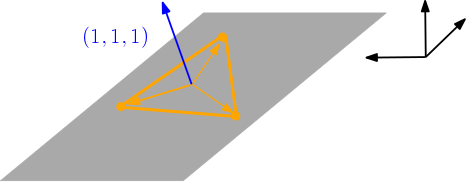
\includegraphics[scale=0.5]{res_embedding}
	\caption{The resistive embedding (in orange;  light) of a graph with three nodes sits in a plane (gray) which is parallel to the all ones vector. }
	\label{fig:res_embedding}
\end{figure}

The relationship between $\re$ and $\splx$ gives us an alternate way to prove equalities such as \eqref{eq:c(S_U)}: There exists an isometry\footnote{A distance preserving map.} between $\re$ and $\splx$, so 
\begin{equation*}
\norm{\cent(\splx^+_U)}_2^2 = \norm{\cent(\re_U)}_2^2 = \frac{1}{|U|^2} \norm{\L_G^{+/2}\bchi_U}_2^2 = \frac{1}{|U|^2}w(\delta^+ U).
\end{equation*}


Additionally, just as $\splx_G^+$  has  the inverse $\splx_G$, $\respol_G$  has an inverse which respects the same  relationships. As one might guess, this inverse has vertex matrix $\L_G^{1/2}$. To see this, for any $i,j\neq k$,  we have 
\begin{equation*}
\la \L_G^{1/2}\bchi_i,\L_G^{+/2}\bchi_j-\L_G^{+/2}\bchi_k\ra = \bchi^\tp \L_G^{1/2}\L_G^{+/2}(\bchi_j-\bchi_k)\ra,
\end{equation*}
where 
\begin{align*}
\L_G^{1/2}\L_G^{+/2} &= \sum_{r,s=1}^{n-1}\lambda_r^{1/2}\lambda_s^{-1/2}\vp_r\vp_r^\tp\vp_s\vp_s^\tp = \sum_{r=1}^{n-1} \vp_r\vp_r^\tp,
\end{align*}
and 
\begin{align*}
\sum_{r=1}^{n-1}\bchi_i \vp_r\vp_r^\tp\bchi_j = \sum_{r=1}^{n-1}\vp_r(i)\vp_r(j) = \delta_{ij} - \frac{1}{n},
\end{align*}
using Equation \eqref{eq:sum_double_ortho}. Hence, 
\begin{align*}
\bchi_i^\tp \L_G^{1/2}\L_G^{+/2}(\bchi_j-\bchi_k) = \delta_{ij} - \frac{1}{n} - (\delta_{ik}-\frac{1}{n}) = \delta_{ij}.
\end{align*}

\note{Still investigating this relationship and its properties.}



\section{Random Walks}
In this section we briefly highlight a few connections between stochastic process on $G$ and  the geometry of its inverse combinatorial simplex $\splx_G^+$. 

First  we  note that the total effective resistance translates to the total pairwise distance in the simplex: 
\begin{align}
\Rtot_G = \frac{1}{2}\sum_{i,j\in[n]} \effr(i,j) = \frac{1}{2}\sum_{i,j\in[n]}\norm{\sv_i^+-\sv_j^+}_2^2. \label{eq:rtot_simplex}
\end{align}
This connection gives us a new way to prove certain identities. For example, 
\begin{align*}
\sum_{i,j\in[n]}\norm{\sv_i^+-\sv_j^+}_2^2 &= n\sum_{in[n]}\norm{\sv_i^+}_2^2 + n\sum_{j\in[n]}\norm{\sv_j^+}_2^2 - 2\sum_{i,j\in[n]}\la\sv_i^+,\sv_j^+\ra \\ 
&= n\sum_{\in[n]}\L_G^+(i,i) + n\sum_{j\in[n]}\L_G^+(j,j) - 2\sum_{i\in[n]}\la \L_G(i,\cdot),\one\ra = 2n\Tr(\L_G^+),
\end{align*}
since $\L_G^+\one=\zero$. 
Hence, by \eqref{eq:rtot_simplex},
\begin{equation*}
\Rtot_G=n\Tr(L_G^+) = n\sum_{i\in[n]}\sum_{j<n} \frac{1}{\lambda_i}\vp_i(j)^2 =\sum_{j<n}\frac{1}{\lambda_j}\norm{\vp_j}_2^2 = \sum_{j<n}\frac{1}{\lambda_j}.
\end{equation*}
This is of course a well-known equation---originally produced by Klein  and Randi\'{c}~\cite{klein1993resistance}---but the interest resides in the fact that it can be derived via the graph-simplex correspondence.  

We also note that this gives us another tool with  which to compute the effective resistance of certain graphs.  Notice that the computation above immediately leads to $\Rtot_G = n\sum_{i\in[n]}\norm{\sv_i^+}_2^2$. Let $K_n^\alpha$ denote the complete graph on $n$ vertices where each edge has weight $\alpha$. By Corollary~\ref{cor:Lkn+_laplacian}, $\L_{K_n^\alpha}^+=\L_H$ for some graph $H$. Therefore, $\L_{K_n^\alpha}=\L_H^+$ and  $\norm{\sv_i^+(H)}_2^2 = \norm{\sv_i(\L_{K_n^\alpha})}_2^2$.  If $K_n$ is the unweighted complete graph, we see that $\L_{K_n^\alpha}=\alpha\L_{K_n}$. Using  that $L_{K_n}$ has eigenvalue $n$ with multiplicity $n-1$  (Section~\ref{sec:examples}) gives $L_{K_n^\alpha}=\alpha n\sum_{i<n}\vp_i\vp_i^\tp$, meaning that $\L_{K_n^\alpha}=\L_H^+$ has eigenvalue $\alpha n$ with multiplicity $n-1$. The effective resistance of $H$ is then 
\begin{equation*}
\Rtot_H = n\Tr(\L_H^+) = \alpha(n-1). 
\end{equation*}
Moreover, $\L_H$ has eigenvalue $(\alpha n)^{-1}$ with multiplicity $n-1$, and  is therefore a complete graph with weights $(\alpha n^2)^{-1}$. We have proven the  following:  

\begin{lemma}
	For any complete graph $H$ on $n$ vertices with uniform edge weights  $(\alpha n^2)^{-1}$ for any $\alpha$,  $\Rtot_H = \alpha (n-1)$. 
\end{lemma}

\subsection{Continuous Time Random Walks}

In this section  we investigate how a random walk in a hyperacute simplex  is governed by the eigenvalues  and eigenvectors of its associated graph. 
We examine a continuous time random walk \note{Say more about where this comes from} which  obeys the equation 
\begin{equation*}
\frac{d \bpi(t)}{dt } = -\L_G\W_G^{-1/2} \bpi(t),
\end{equation*}
which has the solution $\bpi(t)  = \exp(-\L_G\W_G^{-1/2}t)\bpi(0)$. This, however, is relative unsightful in terms of  analyzing the dynamics of $\bpi(t)$ in terms of the  graph.  Instead, in  what follows we seek  to develop a solution to $\bpi(t)$ in terms of the  eigendecomposition of  $G$.  Define $\bpi_1(t) = \W^{-1/2}\pi(t)$ and $\bpi_2(t) = \Eign^\tp \bpi_1(t)$, where we recall that $\Eign^\tp$ is the eigenvector matrix  of  $\Ln_G$.  Then 
\begin{equation*}
\frac{d \bpi_1(t)}{dt} = \W^{-1/2}\frac{d \bpi(t)}{dt} = -\W^{-1/2}\L_G\W^{-1/2}\W^{-1/2}\bpi(t) = - \Ln_G\bpi_1(t),
\end{equation*}
and, using the eigendecomposition of $\Ln_G$,   
\begin{equation*}
\frac{ d\bpi_2(t)}{dt} = \Eign^\tp \frac{d\bpi_1(t)}{dt} = -\Eign^\tp \Ln_G \bpi_1(t) = -\Eign^\tp \Eign\Evaln\Eign^\tp \bpi_1(t) = -\Evaln  \bpi_2(t),
\end{equation*}
since  $\Eign^\tp\Eign=\I$. This equation  has the solution 
\begin{equation*}
\bpi_2(t) = \exp(-\Evaln t)\bpi_2(0) = \begin{pmatrix}
e^{-\lambda_1 t}  & &\\
& \ddots  & \\
&& e^{-\lambda_{n-1} t}
\end{pmatrix}  \bpi_2(0).
\end{equation*}

\begin{figure}
	\centering
	\begin{minipage}{0.32\textwidth}
		\centering
		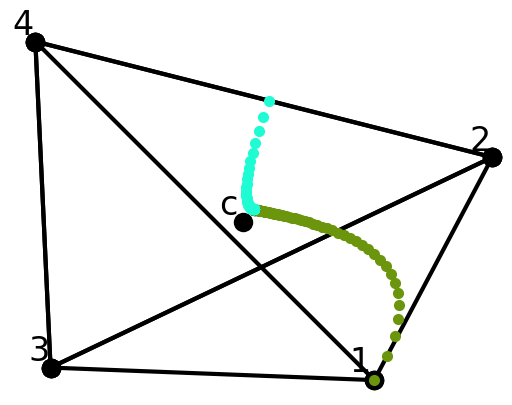
\includegraphics[scale=0.6]{dynamics1}
		\subcaption{}
	\end{minipage}
	\begin{minipage}{0.32\textwidth}
		\centering
		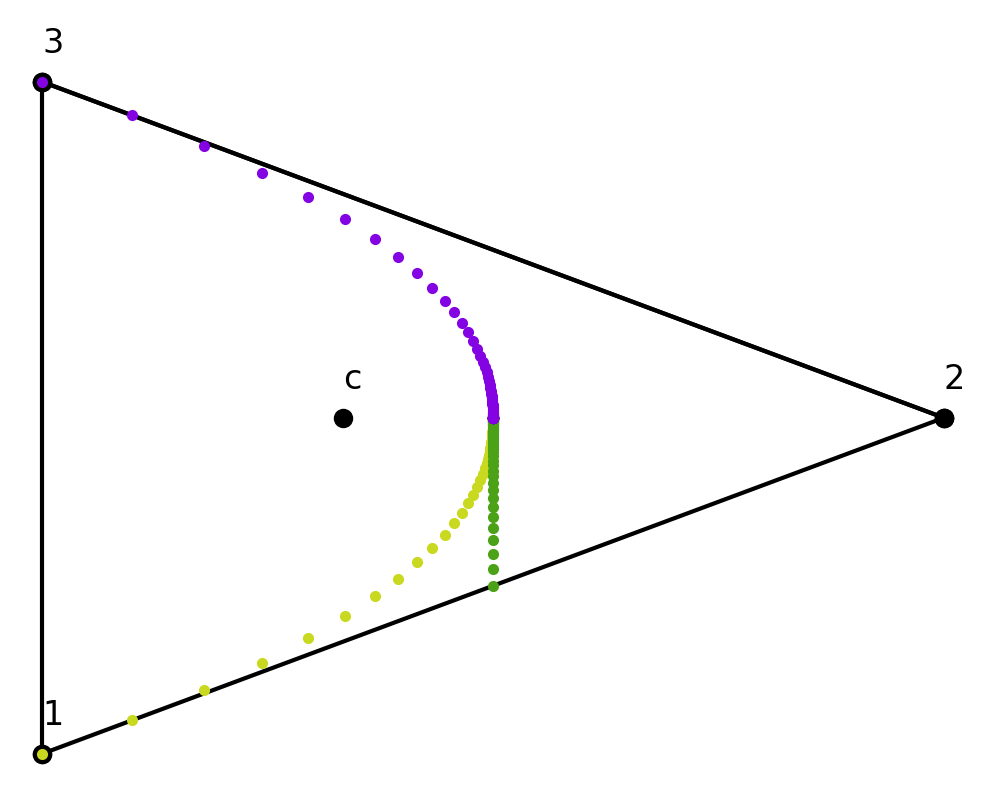
\includegraphics[scale=0.4]{dynamics3}
		\subcaption{}
	\end{minipage}
	\begin{minipage}{0.32\textwidth}
		\centering
		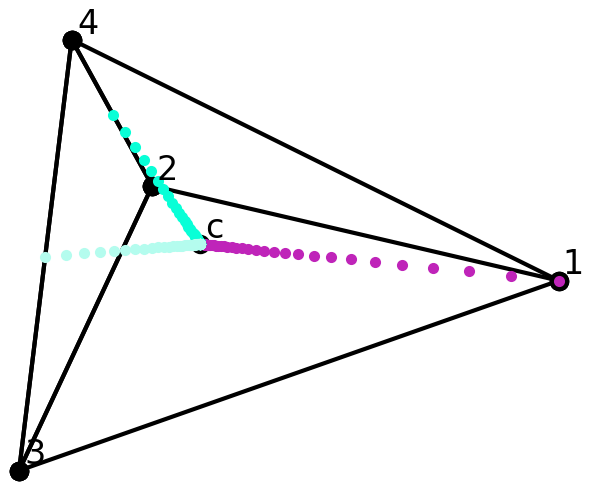
\includegraphics[scale=0.6]{dynamics2}
		\subcaption{}
	\end{minipage}
	\caption{Random walk dynamics plotted as points  in the simplex.}
\end{figure}

Combining the  definitions of $\bpi_1$  and $\bpi_2$ gives $\bpi_2(t)  = \Eign^\tp \bpi_1(t) = \Eign^\tp \W^{-1/2}\bpi(t)$, hence 
$\bpi(t) = \W^{1/2} \Eign \bpi_2(t)$. As a point in the  simplex this gives 
\begin{equation*}
\p(t)  = \Sv\bpi(t) = \Eval^{1/2}\Eig^\tp \W^{1/2}\Eign \bpi_2(t) = \Y\bpi_2(t),
\end{equation*}
after definining $\Y\equiv \Eval^{1/2}\Eig^\tp \W^{1/2}\Eign$. As a point in the normalized simplex, we have 
\begin{equation*}
\q(t) = \Svn\bpi(t) = \Evaln^{1/2}\Eign^\tp\W^{1/2}\Eign\bpi_2(t) = \Yn\bpi_2(t),
\end{equation*}
where $\Yn= \Evaln^{1/2}\Eign^\tp\W^{1/2}\Eign$. We thus  see that the matrices 
\begin{equation*}
\Y = \begin{pmatrix}
\lambda_1^{1/2}\sum_{i\in[n]} \vp_1(i)\vpn_1(i) w_i^{1/2} & \dots &  \lambda_1^{1/2}\sum_{i\in[n]} \vp_1(i)\vpn_{n-1}(i) w_i^{1/2} \\
\vdots & \ddots & \vdots \\
\lambda_{n-1}^{1/2}\sum_{i\in[n]} \vp_{n-1}(i)\vpn_1(i) w_i^{1/2} & \dots &  \lambda_{n-1}^{1/2}\sum_{i\in[n]} \vp_{n-1}(i)\vpn_{n-1}(i) w_i^{1/2} 
\end{pmatrix},
\end{equation*}
and  
\begin{equation*}
\Yn  = \begin{pmatrix}
\lambdan_1^{1/2}\sum_{i\in[n]} \vpn_1(i)\vpn_1(i) w_i^{1/2} & \dots &  \lambdan_1^{1/2}\sum_{i\in[n]} \vpn_1(i)\vpn_{n-1}(i) w_i^{1/2} \\
\vdots & \ddots & \vdots \\
\lambdan_{n-1}^{1/2}\sum_{i\in[n]} \vpn_{n-1}(i)\vpn_1(i) w_i^{1/2} & \dots &  \lambdan_{n-1}^{1/2}\sum_{i\in[n]} \vpn_{n-1}(i)\vpn_{n-1}(i) w_i^{1/2} 
\end{pmatrix},
\end{equation*}
govern the dynamics of the random walk in  $\splx_G$ and $\splxn_G$, respectively.  More specifically, letting $\Y=(\y_1\;\dots\;\y_n)$ we have 
\[\p(t) = \sum_{i\in[n-1]} \y_i (\bpi_2(t))(i) = \sum_{i\in[n-1]}  \y_i e^{-\lambda_i t} \Eign^\tp \W^{-1/2}\bpi(0)(i).\]







